\chapter{International Data Transfers in Anycast Ecosystems}
\label{ch:experiments}

The previous chapter introduced Hunter, a methodology capable of inferring the geographic destinations of anycast communications through active network measurements and latency-based multilateration techniques. While the validation results demonstrated the feasibility and reliability of the proposed approach, the actual impact of anycast infrastructures on data protection and data sovereignty remains an open question. In particular, it is necessary to understand whether modern Internet services effectively produce international transfers of personal data that remain unknown to users, developers, and regulatory transparency mechanisms.

Mobile ecosystems constitute a particularly suitable environment for analysing this phenomenon due to their global scale, the central role they play in users' daily activities, and their extensive dependence on external network services. Modern smartphones continuously interact with remote infrastructures to provide functionalities such as content synchronisation, analytics, advertising, authentication, notifications, or multimedia delivery. As a consequence, mobile devices generate a large volume of network communications involving multiple service providers and potentially jurisdictions.

The Android ecosystem is especially appropriate for this analysis because of its worldwide adoption, the openness of its application distribution model, and the extensive use of Third-Party Libraries (TPLs). Android applications rarely operate as isolated software components and instead integrate external SDKs and services responsible for analytics, advertising, crash reporting, authentication, content delivery, or user tracking functionalities. These libraries could establish communications independently from the application developer, frequently without explicit visibility regarding the final infrastructure receiving the transmitted data.

From a regulatory perspective, this lack of geographic transparency introduces substantial challenges. Modern privacy regulations such as the GDPR \cite{REGULATIONSRelevance} impose strict obligations regarding international transfers of personal data, including transparency requirements concerning the jurisdictions where data may be processed or accessed. However, anycast infrastructures fundamentally decouple logical service identifiers from physical geographic destinations. Consequently, the jurisdictions effectively reached by Internet communications may differ from those declared in privacy policies or assumed by service providers.

This chapter presents a large-scale empirical analysis of international data transfers performed through anycast infrastructures within the Android ecosystem. Using Hunter as the core geographic inference mechanism, the study analyses the destinations reached by anycast communications generated by Android applications and their embedded TPLs. The objective is twofold. First, the chapter seeks to quantify the prevalence of international data transfers associated with anycast communications and characterise their geographic behaviour. Second, it evaluates whether the observed destinations align with the transparency obligations established by current data protection frameworks, particularly the GDPR.

The analysis is structured progressively. First, the experimental methodology used for traffic collection, privacy policy analysis, and geographic inference is presented. Next, the chapter analyses the existence of cross-border personal data transfers triggered by anycast communications in Android applications, including their temporal variability and the prevalence of destinations located outside the EEA. Afterwards, the observed destinations are compared against the jurisdictions declared in privacy policies in order to evaluate transparency and disclosure compliance. The role of TPLs as one of the main drivers of these communications is then analysed in detail. Finally, the chapter extends the discussion beyond the Android ecosystem and presents a broader perspective on jurisdictional exposure in operational anycast infrastructures, motivating the need for deterministic geographic control mechanisms discussed in subsequent chapters.

\section{Experimental Methodology}
\label{sc:anycast_experiments_methodology}

This chapter presents a large-scale empirical analysis of international data transfers performed through anycast infrastructures in the Android ecosystem. The objective of the experimental methodology is to observe the anycast communications generated by Android applications and their embedded Third-Party Libraries (TPLs), infer the geographic destinations reached by these communications using Hunter, and compare the observed jurisdictions with the information disclosed in the corresponding privacy policies.

The methodology combines dynamic traffic analysis, active network measurements, and automatic inspection of privacy policies in order to characterise both the technical and regulatory dimensions of the problem. Figure~\ref{fig:experiment_tpls_analysis_workflow} summarises the overall workflow followed during the experiments.

\begin{figure}
    \centering
    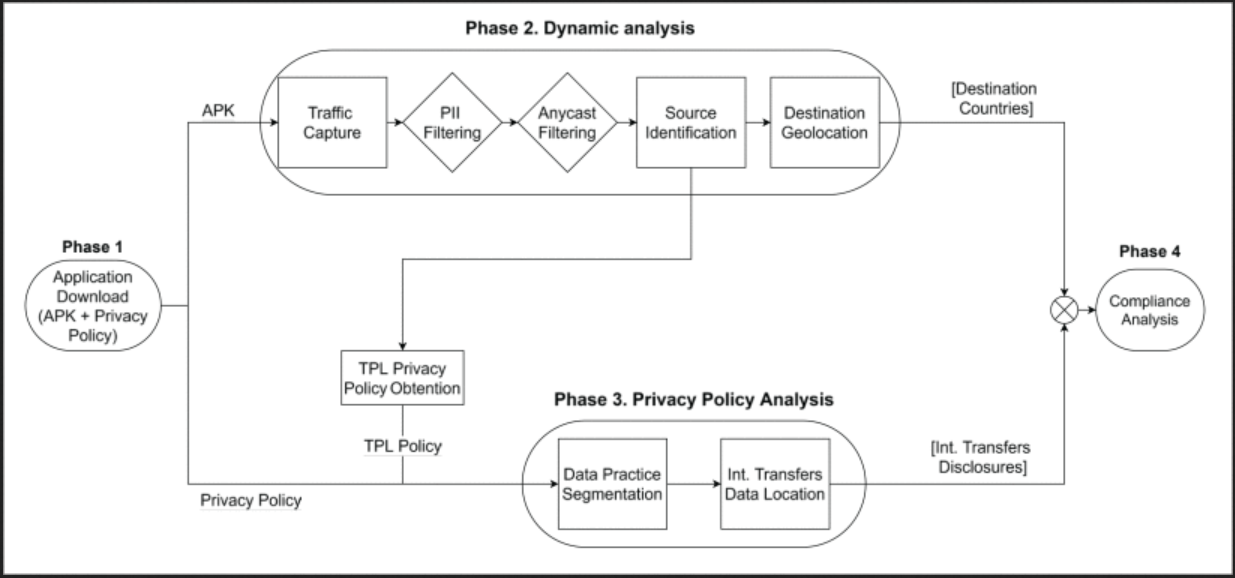
\includegraphics[width=\textwidth]{figures/images/experiment_tpls_analysis_workflow.png}
    \caption{Overview of the experimental methodology used to analyse international data transfers in Android applications.}
    \label{fig:experiment_tpls_analysis_workflow}
\end{figure}

\subsection{Application Selection and Dataset Construction}
\label{sc:anycast_experiments_dataset}

The experimental analysis was conducted using a large-scale corpus of Android applications collected from the Google Play Store. The objective of the dataset construction process was to obtain a representative sample of widely deployed mobile applications actively used by end users and strongly dependent on cloud infrastructures and external online services.

Initially, 6,000 popular Android applications with more than 100,000 downloads were randomly selected from the Google Play Store \cite{Pascual2025AnycastDisaster}. The selected applications covered multiple categories of the Android ecosystem, including communication, entertainment, productivity, finance, gaming, shopping, and social networking applications. This diversity aimed to capture a broad representation of the current Android application ecosystem and its associated communication behaviours.

For each selected application, both the APK installation package and the associated privacy policy were automatically collected. APK files were downloaded from the Google Play Store using the API described in \cite{Marty0678/googleplay-api:API}. Privacy policies were retrieved by scraping the corresponding application pages available on the Google Play Store, where developers are required to provide a policy link whenever personal data is processed.

Although 6,000 applications were initially selected, only 5,759 applications were successfully processed during the dynamic analysis phase. Some applications refused execution within the experimental environment due to anti-analysis protections, root detection mechanisms, execution failures, or incompatibilities with the instrumentation framework.

The analysed applications exhibit a strong dependence on external cloud infrastructures and embedded Third-Party Libraries (TPLs) responsible for functionalities such as analytics, monetization, crash reporting, advertising, authentication, user tracking, or content delivery. This characteristic makes the Android ecosystem particularly suitable for studying the impact of anycast communications on international data transfers, as a substantial portion of the generated traffic is delegated to infrastructures operating beyond the direct control of application developers.

\subsection{Dynamic Traffic Analysis}
\label{sc:anycast_experiments_traffic_collection}

The second phase of the methodology focuses on executing the collected applications and analysing the network traffic generated during their operation in order to identify communications containing personal data and directed towards anycast infrastructures.

This phase builds upon a previously developed and validated framework and combination techniques for large-scale privacy analysis in Android ecosystems \cite{Guaman2023AutomatedApplications}. In particular, the application execution environment, traffic interception infrastructure, execution trace collection mechanisms, and personal data identification techniques were inherited from this previous work. Therefore, only the aspects directly relevant to the present study are summarised here.

The applications were executed on real Android devices within a controlled analysis environment. Each application was initially launched and manually interacted with for two minutes in order to initialise its execution and trigger realistic user-driven behaviours. Subsequently, the Android Monkey testing tool \cite{IUDevelopers} was used for three additional minutes to automatically stimulate the application and explore additional execution paths and communication behaviours.

During execution, the generated network traffic was intercepted through a man-in-the-middle TLS interception proxy capable of inspecting HTTPS communications. This infrastructure enabled the extraction of destination domains, remote IP addresses, HTTP metadata, and application-layer payloads associated with the observed connections.

In parallel, an instrumentation component deployed on the Android devices collected execution traces from the running applications. These traces preserve package-level information regarding the code responsible for triggering each communication, enabling the identification of the embedded TPLs associated with the observed traffic.

The captured communications were subsequently analysed to identify transmissions containing personal data according to the GDPR interpretation guidelines provided by the European Union \cite{JUSTICEwp260rev.01}. The detected personal data types include device identifiers, advertising identifiers, hardware information, operating system metadata, coarse and precise location information, and network information, such as the WiFi BSSIDs to which the device is connected and MAC addresses.

The performed dynamic analysis intercepted a total of 4,278,823 communications generated by the analysed applications. Among them, 242,497 communications contained personal data. The collected traffic was subsequently filtered to retain only communications satisfying two simultaneous conditions: containing personal data and targeting anycast destination IP addresses. After applying these filters, the resulting dataset consisted of 195,786 communications directed towards 200 anycast IP addresses originating from 960 different Android applications \cite{Pascual2025AnycastDisaster}.

To determine whether a destination IP address belonged to anycast infrastructure, the methodology relied on publicly available datasets and commercial classification services, including the MAnycast2 census \cite{Sommese2020MAnycast2:Anycast} and the IPInfo commercial database \cite{IPIPinfo}. These sources provide classifications and routing-related information that enable the identification of operational anycast deployments. In particular, IPInfo explicitly annotates whether an IP address belongs to an anycast infrastructure, which enabled the filtering of communications directed towards anycast services during the analysis.

The execution traces additionally enabled the identification of embedded TPLs responsible for many of the observed communications. In total, 20 distinct TPLs were identified as triggering 61,443 communications containing personal data and directed towards anycast infrastructures.

As with any large-scale dynamic analysis methodology, the proposed approach presents inherent limitations. Dynamic execution cannot guarantee complete behavioural coverage, particularly for functionalities requiring complex user interactions, authentication processes, or external conditions that may not be reproducible within the experimental environment. Consequently, the obtained results should be interpreted as a lower bound of the actual phenomenon rather than as an exhaustive enumeration of all possible communications performed by the analysed applications.

\subsection{Privacy Policy and Third-Party Library Analysis}
\label{sc:anycast_experiments_privacy_policies}

The third phase of the methodology focuses on analysing the privacy policies associated with both the Android applications and the embedded TPLs in order to evaluate the transparency of the observed international communications.

For each analysed application, the corresponding privacy policy text was automatically collected during the dataset acquisition phase. The policy texts were subsequently processed using machine learning and natural language processing techniques to identify references related to international data transfers, third-party data sharing practices, and the countries where personal data may potentially be processed or accessed.

Particular attention was devoted to extracting the set of countries explicitly disclosed in the privacy policies as potential destinations for international personal data transfers. These disclosed jurisdictions were later compared against the actual geographic destinations of the anycast communications inferred through Hunter.

The same analysis was conducted for the privacy policies associated with the identified TPLs. However, unlike application privacy policies, TPL privacy documentation frequently lacks standardised publication formats or consistent accessibility mechanisms. Consequently, the collection and verification of TPL privacy policies required partial manual intervention during the analysis process.

The analysis performed revealed a highly heterogeneous transparency landscape. Some applications explicitly disclosed destination countries and international transfer mechanisms, while many others only provided generic references to international processing, cloud infrastructures, or external service providers without specifying the actual jurisdictions involved in the observed communications.

A similar situation was observed among TPLs. Several libraries either lacked publicly accessible privacy policies or failed to explicitly identify the countries associated with their international data processing activities, despite generating communications towards anycast infrastructures located outside the European Economic Area (EEA).

The comparison between the jurisdictions declared in privacy policies and the destinations empirically inferred through network measurements enabled the identification of applications and TPLs potentially failing to satisfy GDPR transparency requirements regarding international transfers of personal data.

\subsection{Anycast Destination Inference}
\label{sc:anycast_experiments_hunter_integration}

The final phase of the methodology focuses on determining the geographic destinations associated with the identified anycast communications. Since the destination reached by an anycast communication depends on the origin network and the dynamic state of Internet routing, identifying the physical location of the serving infrastructure requires active network measurements and geographic inference techniques. To address this problem, the experiments leveraged Hunter, the methodology presented in Chapter~\ref{ch:hunter}. Hunter combines traceroute analysis, last-hop identification, latency-based multilateration, and country inference techniques to estimate the physical destination country associated with communications towards anycast infrastructures.

For each anycast IP address identified during the dynamic analysis phase, distributed measurements were executed from geographically distributed vantage points across the EEA using RIPE Atlas probes \cite{HomeAtlas}. The experiments focused on EEA countries because the GDPR establishes explicit transparency and adequacy requirements regarding international transfers of personal data outside the EEA jurisdictional space.

The source probes were selected by dividing the EEA territory into geographic cells of three degrees of latitude and longitude. For each cell, a random RIPE Atlas probe belonging to an EEA country was selected. Approximately 110 probes were used during each measurement campaign, providing broad geographic coverage across the EEA.

For every source probe and anycast IP pair, Hunter inferred the destination country reached by the communication. The measurements were repeated ten times for each IP in order to capture routing variability and identify potential changes in the selected anycast replica caused by network fluctuations, BGP routing dynamics, or traffic engineering mechanisms.

The results produced by Hunter were subsequently correlated with the traffic analysis and privacy policy datasets. This integration enabled the systematic identification of Android applications and TPLs generating communications towards anycast infrastructures located outside the EEA, as well as the evaluation of whether these international destinations were transparently disclosed in the corresponding privacy policies.

\section{Cross-border Communications in Android Applications}
\label{sc:anycast_experiments_cross_border}

\subsection{Observed International Transfers}
\label{sc:anycast_experiments_observed_transfers}

The large-scale analysis of Android applications revealed a widespread use of anycast infrastructures for communications involving personal data. From the initial dataset of 6,000 applications, 5,759 were successfully analysed, generating a total of 4,278,823 network communications during the dynamic analysis phase.

Among these communications, 242,497 were identified as containing personal data according to the criteria described in Section~\ref{sc:anycast_experiments_traffic_collection}. The subsequent analysis of destination addresses showed that a substantial fraction of these communications relied on anycast infrastructures. After filtering the collected traffic to retain only communications simultaneously containing personal data and targeting anycast IP addresses, the resulting dataset consisted of 195,786 communications, representing 80.74\% of all communications containing personal data, directed towards 200 distinct anycast IP addresses.

These communications were generated by 960 different Android applications, indicating that the use of anycast infrastructures for processing personal data is not restricted to a small number of services or application categories. Instead, the phenomenon appears across a broad spectrum of applications and online services deployed within the Android ecosystem.

The analysis further showed that communications towards anycast infrastructures are frequently associated with the collection and transmission of device identifiers, advertising identifiers, hardware characteristics, operating system information, and location-related data. Consequently, anycast infrastructures were commonly present in communication flows carrying personal data generated by modern Android applications.

\subsection{Temporal and Geographic Variability}
\label{sc:anycast_experiments_variability}

\hugo{Include number of origins with variability, mean of destinations by IP and origin.}

One of the most distinctive characteristics of anycast infrastructures is that the destination reached by a communication is not solely determined by the destination IP address. Instead, the selected server depends on the routing decisions made by the network, which are influenced by factors such as the geographic origin of the communication, BGP policies, peering agreements, traffic engineering mechanisms, and transient network conditions.

The measurements performed during the experiments confirmed that this behaviour is common among operational anycast deployments. For many of the analysed anycast IP addresses, communications originating from different EEA countries reached different destination countries despite targeting the same IP address. Consequently, the set of destinations potentially involved in an anycast communication cannot be determined solely from the destination address itself.

In addition to geographic variability, the experiments also revealed temporal variability. Repeated executions of Hunter against the same anycast IP occasionally produced different destination countries even when the origin country remained unchanged. This behaviour reflects the dynamic nature of Internet routing, where modifications in network conditions, routing policies, congestion levels, or traffic engineering decisions may alter the anycast replica selected to serve a communication.

To capture this phenomenon, the destination inference process was repeated ten times for each source-destination pair. This repeated measurement strategy enabled the identification of destination countries that may only appear under specific network conditions and reduced the risk of drawing conclusions from transient routing states.

The observed variability demonstrates that anycast infrastructures should not be understood as providing a single geographic destination. Instead, a communication directed towards an anycast IP address may potentially reach different countries depending on when and from where the communication is initiated. Therefore, analysing only a single measurement or a single geographic origin would provide an incomplete view of the actual geographic exposure associated with anycast communications.

This behaviour has important implications for understanding the geographic footprint of Internet services. Rather than being associated with a single jurisdiction, many anycast deployments exhibit a set of potential destinations whose composition may vary over time, making the geographic behaviour of the service inherently dynamic.

\subsection{Destinations Outside the EEA}
\label{sc:anycast_experiments_non_eea}

\hugo{Include examples in order to reinforce the claimed situations.}

After identifying the destination countries associated with the analysed anycast communications, the results were filtered to study those involving transfers of personal data towards countries located outside the European Economic Area (EEA).

The analysis revealed that international transfers outside the EEA are far from exceptional. Among the 200 anycast IP addresses identified during the experiments, 195 were associated with at least one destination located outside the EEA. This indicates that communications carrying personal data towards anycast infrastructures frequently cross jurisdictional boundaries despite originating from users located within the EEA.

The inferred destinations outside the EEA included the United Kingdom, Switzerland, the United States, Ukraine, Serbia, and Russia. Figures~\ref{fig:transfers_outside_EEA}, \ref{fig:transfers_from_EEA_to_UK_and_SW}, and \ref{fig:transfers_from_EEA_to_RU_and_more} illustrate the geographic distribution of these transfers and the countries involved.

\begin{figure}
    \centering
    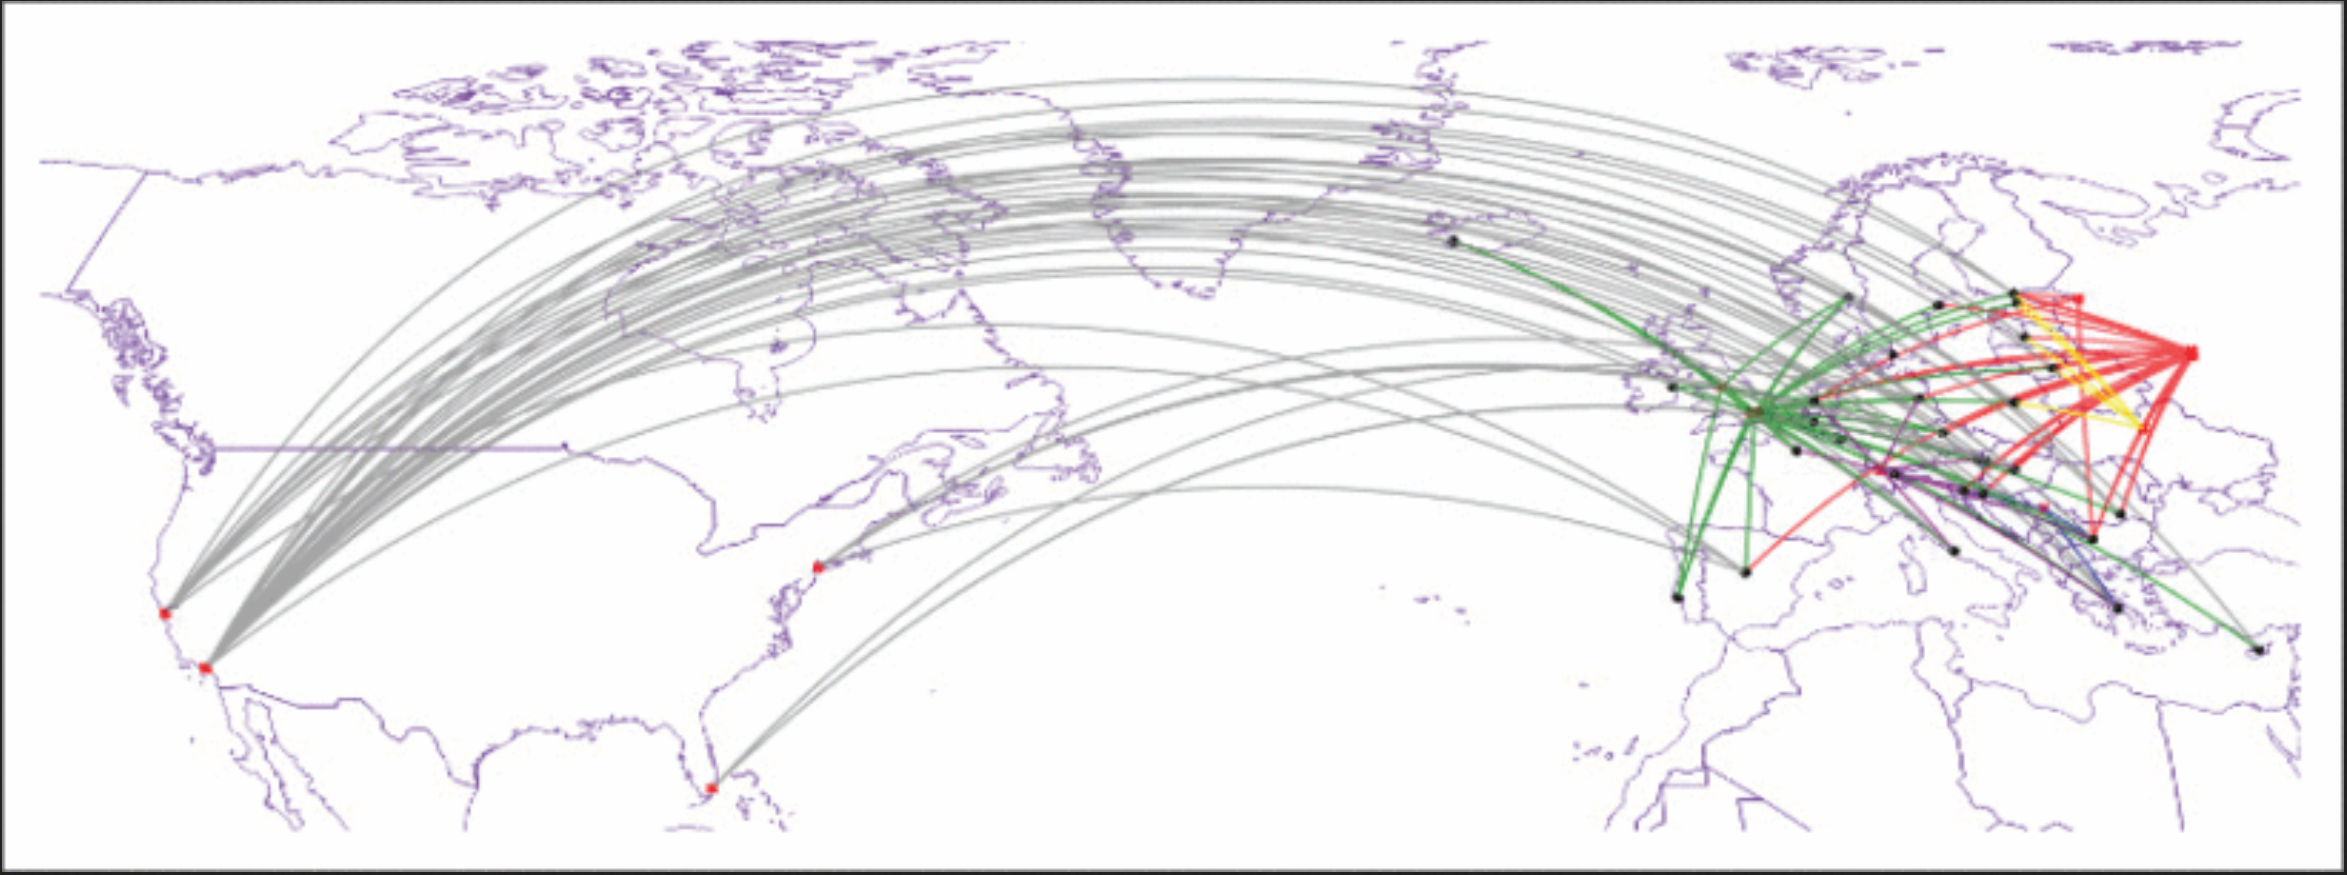
\includegraphics[width=\textwidth]{figures/images/transfers_outside_EEA.png}
    \caption{International transfers from EEA countries to non-EEA destinations.}
    \label{fig:transfers_outside_EEA}
\end{figure}

\begin{figure}
    \centering
    \begin{subfigure}[t]{0.48\textwidth}
        \centering
        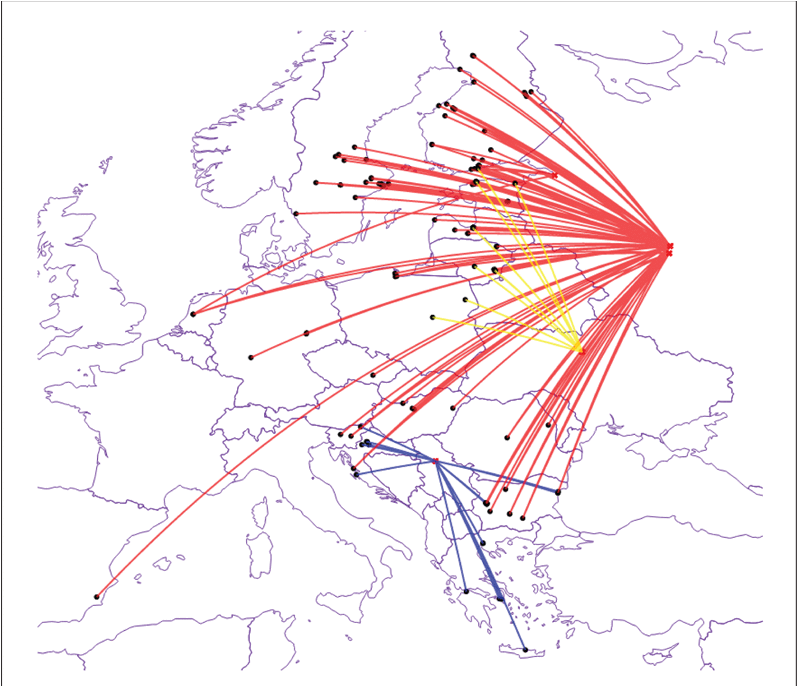
\includegraphics[width=\textwidth]{figures/images/transfers_from_EEA_to_RU_and_more.png}
        \caption{International transfers from EEA countries to anycast servers in Ukraine (yellow), Serbia (blue) and Russia (red).}
        \label{fig:transfers_from_EEA_to_RU_and_more}
    \end{subfigure}
    \hfill
    \begin{subfigure}[t]{0.48\textwidth}
        \centering
        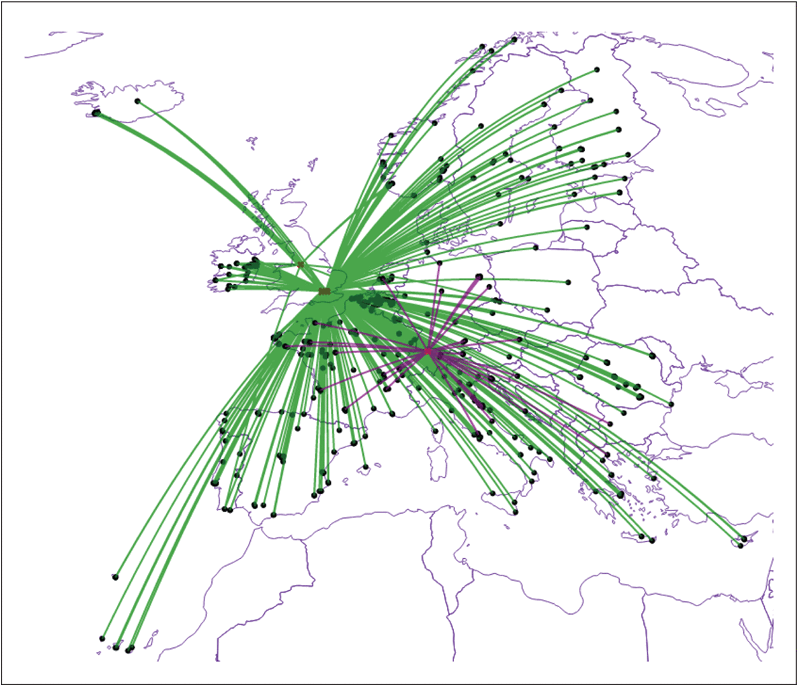
\includegraphics[width=\textwidth]{figures/images/transfers_from_EEA_to_UK_and_SW.png}
        \caption{International transfers from EEA countries to anycast servers in United Kingdom (green) and Switzerland (purple).}
        \label{fig:transfers_from_EEA_to_UK_and_SW}
    \end{subfigure}
    \caption{International transfers from EEA countries to non-EEA destinations identified during the experiments.}
    \label{fig:transfers_non_eea}
\end{figure}

The results show that transfers towards neighbouring non-EEA countries were particularly common. The United Kingdom and Switzerland appeared frequently as destinations for communications originating from multiple EEA countries. This behaviour is consistent with the geographic distribution of many anycast deployments, where traffic is commonly directed towards the nearest operational replica regardless of political or regulatory boundaries.

More concerningly, the analysis also identified transfers towards countries located significantly further from the communication origin, including the United States, Serbia, Ukraine, and Russia. These observations demonstrate that geographic proximity alone cannot be assumed when reasoning about the destination of communications directed towards anycast infrastructures.

The obtained results additionally revealed that the set of reachable destination countries varies depending on the origin country. The same anycast IP address may lead to different destination countries when accessed from different locations within the EEA, reinforcing the idea that anycast communications should be understood as a set of potential geographic destinations rather than a single fixed endpoint.

Overall, the results demonstrate that international transfers outside the EEA are a common characteristic of anycast-enabled services and that the geographic exposure associated with these communications extends well beyond the jurisdictions where the applications themselves are developed or distributed.

\section{Transparency and Privacy Policy Compliance}
\label{sc:anycast_experiments_transparency}

\subsection{Undisclosed International Transfers}
\label{sc:anycast_experiments_undisclosed}

\hugo{Include some reference to the method used for obtaining the privacy policies. In the case of the applications it weas automatic from the Google Play Store, but in the case on the TPLs It has been automatic. Maybe in the first section of obtain the data for the experiment. Include the table of TPLs from the article.}

After identifying the destination countries reached by communications involving personal data, the next step consisted of comparing these empirically observed destinations with the jurisdictions disclosed in the corresponding privacy policies. For each analysed application, the countries inferred through Hunter were contrasted with the list of destinations explicitly mentioned in the application's privacy policy. The same comparison was performed for the privacy policies of the Third-Party Libraries (TPLs) identified as responsible for generating the observed communications.

This comparison revealed a substantial discrepancy between the jurisdictions observed during the experiments and those disclosed to users. While some privacy policies explicitly identified countries where personal data could be processed or transferred, many others only referred to international transfers in generic terms, without specifying the actual destination countries involved.

In numerous cases, privacy policies described the use of cloud providers, content delivery networks, analytics services, or external partners without indicating the jurisdictions where these entities process data. As a result, the information available to users frequently lacked the level of geographic detail required to determine the countries potentially receiving personal data through anycast-enabled communications.

The discrepancy becomes particularly relevant in the context of anycast infrastructures. Since the destination of a communication may vary depending on the origin network and routing conditions, accurately disclosing all possible destination countries is considerably more challenging than in traditional unicast deployments. Nevertheless, from the perspective of the user, the practical consequence remains the same: personal data may be transferred to jurisdictions that are not explicitly mentioned in the privacy documentation.

Among the applications identified as transferring personal data to anycast destinations located outside the EEA, 79.58\% made no explicit mention of international transfers in their privacy policies \cite{Pascual2025AnycastDisaster}. In many cases, the policies only contained generic statements referring to the use of cloud services, external providers, or international operations, without specifying the countries where personal data could ultimately be processed.

When the analysis focused specifically on destination countries, the discrepancy became even more pronounced. The results showed that 98.65\% of the analysed applications potentially failed to satisfy GDPR transparency requirements regarding international transfers, as the countries empirically observed during the experiments were not adequately disclosed in the corresponding privacy documentation \cite{Pascual2025AnycastDisaster}. The situation was similarly concerning for Third-Party Libraries. All identified TPLs were involved in personal data transfers towards anycast infrastructures that could reach destinations outside the EEA. However, 90\% of these libraries potentially failed to disclose the corresponding destination countries despite actively participating in the observed international transfers \cite{Pascual2025AnycastDisaster}.

These findings indicate that users are frequently unable to determine the actual jurisdictions where their personal data may be processed. Even when privacy policies acknowledge the possibility of international transfers, the information provided is often insufficient to effectively identify the countries reached by the communications observed during the experiments. The results also suggest that the lack of transparency cannot be exclusively attributed to application developers. A significant fraction of the observed communications originated from embedded TPLs whose behaviour is often partially opaque to the applications integrating them. Consequently, deficiencies in transfer disclosures may propagate throughout the mobile ecosystem, affecting both application providers and third-party service operators.

\subsection{Limitations of Current Transparency Mechanisms}
\label{sc:anycast_experiments_transparency_limitations}

The observed discrepancies between declared and actual destinations highlight a broader limitation of current transparency mechanisms when applied to modern Internet service infrastructures. Traditional privacy policies are generally written under the implicit assumption that the geographic location of data processing infrastructures is relatively stable and can, therefore, be described through a fixed list of countries or service providers. This assumption becomes increasingly difficult to maintain in environments that rely on anycast deployments.

Unlike conventional unicast infrastructures, anycast systems may route the same communication towards different physical locations depending on the origin network, routing policies, peering relationships, traffic engineering decisions, or temporary network conditions. As a result, the set of countries potentially involved in processing personal data may vary over time, even when users interact with the same service. This dynamic behaviour introduces a fundamental tension between technical reality and regulatory disclosure requirements. Privacy policies are static documents that are typically updated infrequently, whereas the geographic destinations reached through anycast routing may change continuously. Maintaining an exhaustive and accurate description of all possible destinations, therefore, becomes operationally challenging.

The situation is further complicated by the widespread use of Third-Party Libraries and external service providers. Application developers often rely on cloud platforms, analytics providers, advertising networks, and content delivery infrastructures that are managed by independent organisations. Consequently, developers may have limited visibility into the routing behaviour and geographic deployment strategies of the infrastructures ultimately receiving the data.

The results obtained in this study suggest that current transparency mechanisms are poorly adapted to highly distributed Internet architectures. Although privacy policies may disclose the existence of international transfers in general terms, they frequently fail to provide users with sufficient information to determine the jurisdictions that may actually receive their personal data. This limitation does not necessarily imply intentional non-compliance. Rather, it reflects the growing difficulty of reconciling legal transparency obligations with the dynamic and geographically distributed nature of contemporary Internet infrastructures. Nevertheless, from the perspective of users and regulators, the practical consequence remains unchanged: the actual destination countries of personal data transfers often remain unknown.

\section{The Role of Third-Party Libraries}
\label{sc:anycast_experiments_tpls}

\hugo{Include references to the TPLS tables that should be in the previous section.}

The results presented so far show that international transfers through anycast infrastructures are widespread within the Android ecosystem. However, analysing the applications alone provides only a partial view of the phenomenon. A substantial fraction of the observed communications is not generated directly by the application code itself but by Third-Party Libraries (TPLs) integrated into the applications.

Modern Android applications heavily rely on external libraries to provide functionalities such as analytics, advertising, crash reporting, authentication, social network integration, content delivery, and user tracking. Consequently, a significant portion of the personal data collected by applications is ultimately processed through infrastructures operated by organisations other than the application developer. Understanding the role of TPLs is therefore essential to determine how international data transfers emerge within mobile ecosystems and to identify the actors effectively responsible for the observed communications.

The execution traces collected during the dynamic analysis phase enabled the identification of the software components responsible for generating each observed communication. By analysing package names and execution contexts, it was possible to distinguish communications triggered directly by the application from those initiated by embedded TPLs. The results reveal a strong presence of third-party components in the analysed applications. In total, 20 distinct TPLs were identified as responsible for communications involving personal data and anycast infrastructures. These libraries were embedded across a large number of applications belonging to different categories and performing diverse functionalities.

The widespread deployment of TPLs reflects the current structure of the mobile ecosystem, where application developers increasingly delegate specific functionalities to specialised external providers. Rather than implementing analytics, advertising, authentication, or telemetry systems internally, developers often integrate pre-built SDKs that offer these services through a simple programming interface. From a privacy perspective, this delegation has important implications. Although users typically interact with a single application, their personal data may be transmitted to multiple external organisations operating the embedded libraries, or used by them. As a result, understanding data flows within mobile ecosystems requires analysing not only the applications themselves but also the third-party components they incorporate.

In our context, the analysis revealed that TPLs play a central role in the generation of international personal data transfers through anycast infrastructures. Among the 195,786 communications involving personal data and anycast destinations identified during the experiments, 61,443 were directly attributed to embedded TPLs. This result indicates that a significant fraction of the observed communications originated from third-party components operating within the analysed applications. Furthermore, the geographic analysis performed using Hunter showed that all identified TPLs were involved in communications reaching destinations outside the EEA.

This observation is particularly relevant because the deployment strategies adopted by large cloud providers and Internet-scale platforms frequently rely on anycast infrastructures. As a result, a single SDK integrated into hundreds or thousands of applications may generate communications whose destinations vary dynamically according to the geographic origin of the user and the state of the network. The findings, therefore, suggest that TPLs act as major amplifiers of jurisdictional exposure. Through their extensive deployment across the Android ecosystem, a relatively small number of external libraries can influence the geographic destinations reached by personal data originating from a very large number of applications.

The prominent role of TPLs also raises important questions regarding responsibility and transparency in modern mobile ecosystems. From a technical perspective, application developers often have limited visibility into the internal operations of the libraries they integrate. While developers may know the purpose of a given SDK, they frequently lack detailed information regarding the cloud infrastructures used by the provider, the geographic deployment of its services, or the routing mechanisms involved in processing user data. \hugo{Include a mention of the lack of easyness to get the privacy policy, so the application owners can not know directly the privacy policy declares.}

This lack of visibility becomes particularly problematic in the context of anycast infrastructures. Since the destination of a communication may depend on routing decisions that are external to both the application developer and the end user, accurately determining all potential destination jurisdictions becomes significantly more complex. The transparency analysis presented in the previous section illustrates this problem. Although all identified TPLs were involved in international transfers through anycast infrastructures, 90\% of them potentially failed to disclose the destination countries reached by these communications. As a consequence, application developers integrating such libraries may also face difficulties in accurately informing users about the jurisdictions where their data may ultimately be processed.

These findings suggest that the transparency challenges associated with anycast infrastructures cannot be understood solely as an application-level problem. Instead, they emerge from the interaction between application developers, third-party service providers, cloud infrastructures, and Internet routing mechanisms. Consequently, improving transparency regarding international data transfers may require a broader ecosystem-wide approach in which both application developers and TPL providers participate in the disclosure process. Without greater visibility into the geographic behaviour of the infrastructures involved, accurately communicating the potential destinations of personal data transfers remains a challenging task for all actors in the mobile ecosystem.

\section{Global Jurisdictional Exposure in Anycast Systems}
\label{sc:anycast_experiments_global_anycast}

\hugo{Include exact data from the experiment.}

The previous sections demonstrated that Android applications and Third-Party Libraries frequently transfer personal data to anycast infrastructures whose physical destinations may be located in different jurisdictions. However, the observed behaviour is not exclusive to the European region where the previous experiment was conducted; it is a global phenomenon.

To better understand the broader implications of anycast routing, an additional large-scale measurement campaign was conducted using Hunter. Rather than focusing on a specific set of applications, this experiment analysed the geographic destinations reached by anycast infrastructures from a large number of countries and network locations worldwide. The objective was to evaluate the extent to which anycast routing may expose communications to foreign jurisdictions, how stable these routing decisions remain over time, and whether users or organisations can realistically maintain geographic control over the destination of their communications.

The results reveal that jurisdictional exposure is an intrinsic characteristic of operational anycast deployments and not merely a consequence of specific application designs or service providers. Beyond the existence of international routing itself, the measurements revealed a second important phenomenon: the geographic destination of communications varies over time, even when the origin and destination addresses remain unchanged. Repeated measurements showed that identical communications could reach different destination countries depending on the state of the network at the time of the measurement. Variations in BGP routing decisions, traffic engineering mechanisms, peering relationships, congestion management strategies, or changes in the availability of individual replicas may alter the server selected to process a communication.

This behaviour introduces a form of jurisdictional instability in which the legal territory associated with a communication is not fixed but may change dynamically as routing conditions evolve. The instability was particularly evident for infrastructures deployed across multiple neighbouring countries, where relatively small routing changes were sufficient to produce international transfers. In some cases, this cross-border communication also implies a change of jurisdiction, e.g., personal data traffic from the EEA whose destination is Russia or the USA.

These observations highlight a fundamental distinction between anycast and traditional geographically fixed infrastructures. While the physical deployment of servers may remain stable, the jurisdiction effectively reached by a communication can change over time without any visible indication to the user or the application generating the traffic. Consequently, determining the destination jurisdiction of a communication cannot be reduced to a single measurement but instead requires repeated observations capable of capturing the inherent variability of operational anycast deployments.

This dynamic behaviour challenges one of the implicit assumptions underlying many regulatory frameworks: that organisations are able to determine, document, and maintain control over the jurisdictions where personal data are processed. Such an assumption generally holds when communications are directed towards infrastructures deployed in known and geographically stable locations. However, the results obtained in this work suggest that satisfying these requirements becomes considerably more difficult in the presence of anycast routing, where the effective destination of a communication may vary according to network conditions that remain outside the direct control of service providers and end users.

More broadly, the results suggest that geographic location should not be considered a static property of Internet services relying on anycast infrastructures. Instead, geographic destination emerges as a dynamic property influenced by routing behaviour and network conditions. As a consequence, achieving meaningful geographic control over communications requires not only knowledge of where services are deployed but also visibility into how Internet routing selects among the available replicas. These findings reinforce the need for mechanisms capable of continuously assessing the geographic destinations reached by communications and highlight the challenges that anycast infrastructures introduce for data sovereignty, regulatory compliance, and jurisdiction-aware network management.
